\documentclass[oneside]{book}
\usepackage[english]{babel}
\usepackage{amsmath}
\usepackage{framed}
\usepackage{graphicx}
\usepackage{caption}
\usepackage{subcaption}
\usepackage{amsfonts}
\usepackage{amssymb}
\usepackage{float}
\usepackage{xcolor}
\usepackage[toc,page]{appendix}
\usepackage{pythonhighlight}
\usepackage{filecontents}
\usepackage{graphicx}
\usepackage{comment}
\usepackage[english]{babel}
\usepackage{url}
\graphicspath{ {./images/} } 
\DeclareGraphicsExtensions{.png,.pdf}




\begin{document}

\begin{titlepage}
\title{Project DL Course}
\author{Marco Acerbis, Nicolaas Ruberg}

\begin{Huge}
\begin{center}
Project DL Course
\end{center}
\end{Huge}

\begin{large}
\begin{minipage}{2in}
\textbf{project by:} \\
Marco Acerbis \\
Nicoolas Ruberg
\end{minipage}
\hfill
\end{large}

\end{titlepage}

\tableofcontents

\chapter*{Introduction}
\addcontentsline{toc}{chapter}{Introduction}

\chapter{Face Orientation Classification}
\section{VGG19}
VGG19

\section{MobileNet + Clustering}
MobileNet + Clustering

\section{CNN from the Scratch}
CNN from the Scratch

\subsection{Experiment setup}
Our Convolution Neural Network experiment was conducted using "Google Colab", with a GPU machine.
This is the GPU characteristic capture during the execution time.

\begin{comment}
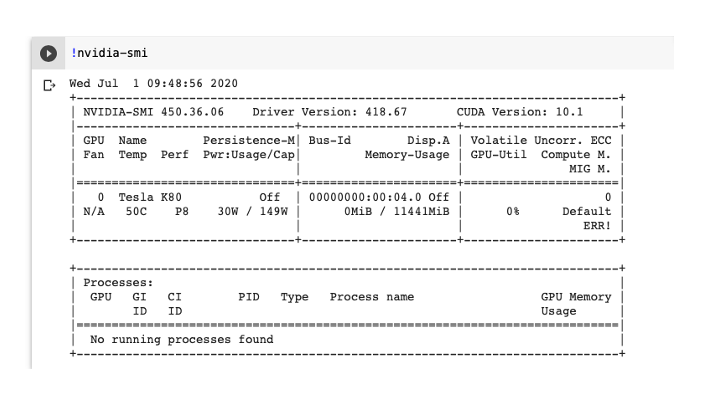
\includegraphics[scale=0.5,bb=0 0 30 30]{GPU}
[width=3cm, height=4cm]
\end{comment}

\begin{small}
\begin{verbatim}
Wed Jul  1 10:25:45 2020
---------------------------------------------------------------------------+
NVIDIA-SMI 450.36.06    Driver Version: 418.67       CUDA Version: 10.1
+----------------------------+----------------------+----------------------+
GPU  Name        Persistence-M  Bus-Id        Disp.A   Volatile Uncorr. ECC
Fan  Temp  Perf  Pwr:Usage/Cap          Memory-Usage   GPU-Util  Compute M.
                                                                     MIG M.
=============================+======================+======================
 0  Tesla K80           Off    00000000:00:04.0 Off                      0
N/A   35C    P8    26W / 149W        0MiB / 11441MiB        0%      Default
                                                                       ERR!
+----------------------------+----------------------+----------------------+
\end{verbatim}
\end{small}

\begin{small}
\begin{verbatim}

Now we can observe the CPU characteristics of the Colab Machine

Architecture:        x86_64
CPU op-mode(s):      32-bit, 64-bit
Byte Order:          Little Endian
CPU(s):              2
On-line CPU(s) list: 0,1
Thread(s) per core:  2
Core(s) per socket:  1
Socket(s):           1
NUMA node(s):        1
Vendor ID:           GenuineIntel
CPU family:          6
Model:               79
Model name:          Intel(R) Xeon(R) CPU @ 2.20GHz
Stepping:            0
CPU MHz:             2200.000
BogoMIPS:            4400.00
Hypervisor vendor:   KVM
Virtualization type: full
L1d cache:           32K
L1i cache:           32K
L2 cache:            256K
L3 cache:            56320K
NUMA node0 CPU(s):   0,1

\end{verbatim}
\end{small}

Next we present the Convolution Neural Network develop to analyze the Celeba Images. We have chosen to take the whole resolution of image as the input of the Network. The strategy devised was inspired on the experiment from \cite{4CNN} with the FashinMinst dataset.

We also change the Drop to 0.7

\begin{figure}[ht]
\caption{Convolution Neural Network with 4 layers)}
\includegraphics[width=10cm, height=16cm]{cnn4}
\centering
\end{figure}


\subsection{First Analyzes}

We ran an experiment with a training set of 8.383 images and a validation set of 1.181 images, for the three categories (pose left, pose front and pose right).
\begin{small}
\begin{verbatim}
Found 8383 images belonging to 3 classes.
Found 1811 images belonging to 3 classes.
\end{verbatim}
\end{small}

\begin{figure}[ht]
\includegraphics[width=8cm, height=6cm]{plot_history}
\centering
\end{figure}


\chapter{Light Source Origin Classification}

\section{Technique 1}
Technique 1

\section{Technique 2}
Technique 2

\chapter{Conclusions}

\addcontentsline{toc}{chapter}{References}
\begin{thebibliography}{9}
\bibitem{Paper by professor Caio}
Dr. Caio;
\textit{Super Awesome Paper for CNNs}, University of Toronto, March 13 2020.

\bibitem{4CNN}
James Le;
\textit{Trained an even deeper CNN classifier with 4 convolution layers}, Github checked on 1st of July 2021.


\end{thebibliography}
\end{document}
